%%%%%%%%%%%%%%%%%%%%%%%%%%%%%%%%%%%%%%%%%%  不使用 authblk 包制作标题  %%%%%%%%%%%%%%%%%%%%%%%%%%%%%%%%%%%%%%%%%%%%%%
%-------------------------------PPT Title-------------------------------------
\title{14-固体光学性质与电子带间跃迁}
%-----------------------------------------------------------------------------
%----------------------------Author & Date------------------------------------

%\author[\textrm{Jun\_Jiang}]{姜\;\;骏\inst{}} %[]{} (optional, use only with lots of authors)
%% - Give the names in the same order as the appear in the paper.
%% - Use the \inst{?} command only if the authors have different
%%   affiliation.
%\institute[BCC]{\inst{}%
\institute[Gain~Strong]{\inst{}%
%\vskip -20pt 北京市计算中心}
\vskip -20pt {\large 格致斯创~科技}}
\date[\today] % (optional, should be abbreviation of conference name)
{%	{\fontsize{6.2pt}{4.2pt}\selectfont{\textcolor{blue}{E-mail:~}\url{jiangjun@bcc.ac.cn}}}
\vskip 45 pt {\fontsize{8.2pt}{6.2pt}\selectfont{%清华大学\;\;物理系% 报告地点
	\vskip 5 pt \textrm{2023.06.10}}}
}

%% - Either use conference name or its abbreviation
%% - Not really information to the audience, more for people (including
%%   yourself) who are reading the slides onlin%%   yourself) who are reading the slides onlin%%   yourself) who are reading the slides onlineee
%%%%%%%%%%%%%%%%%%%%%%%%%%%%%%%%%%%%%%%%%%%%%%%%%%%%%%%%%%%%%%%%%%%%%%%%%%%%%%%%%%%%%%%%%%%%%%%%%%%%%%%%%%%%%%%%%%%%%

\subject{}
% This is only inserted into the PDF information catalog. Can be left
% out.
%\maketitle
\frame
{
%	\frametitle{\fontsize{9.5pt}{5.2pt}\selectfont{\textcolor{orange}{“高通量并发式材料计算算法与软件”年度检查}}}
\titlepage
}
%-----------------------------------------------------------------------------

%------------------------------------------------------------------------------列出全文 outline ---------------------------------------------------------------------------------
\section*{}
\frame[allowframebreaks]
{
  \frametitle{Outline}
%  \frametitle{\textcolor{mycolor}{\secname}}
  \tableofcontents%[current,currentsection,currentsubsection]
}
%%在每个section之前列出全部Outline
%%类似的在每个subsection之前列出全部Outline是\AtBeginSubsection[]
%\AtBeginSection[]
%{
%  \frame<handout:0>%[allowframebreaks]
%  {
%    \frametitle{Outline}
%%全部Outline中,本部分加亮
%    \tableofcontents[current,currentsection]
%  }
%}

%-----------------------------------------------PPT main Body------------------------------------------------------------------------------------
\small
%\section{\rm{VASP~}软件中\rm{PAW~}计算的实现}
%\frame
%
%	\frametitle{\textrm{VASP}计算的特色}
%	相比于与普通的第一原理计算软件,\textrm{VASP}很好地平衡了计算效率和精度的问题,总的来说,\textrm{VASP}主要通过这几个特色保证了计算的高效能
%	\begin{itemize}
%	     \item 迭代与优化算法的多样性\\
%		     本质上电荷密度迭代 \textrm{\&\&} 体系总能量优化是相同的优化问题,采用了类似的算法\upcite{CMS6-15_1996,PRB54-11169_1996}:\\
%			\textcolor{blue}{\textrm{Pseudo-Newton、Conjugate-Gradient、Broyden~mix、damping-factor、RMM-DIIS}}
%	     \item 尽可能采用局域基(原子轨道基)函数:~\\
%		     \textcolor{blue}{\textrm{LREAL}}=\textcolor{red}{\textrm{.TRUE.}}\\
%			优化的投影函数也尽可能在实空间表示
%	     \item \textrm{PAW}原子数据集:\textcolor{blue}{优异的赝势}\upcite{PRB59-1758_1999}
%	\end{itemize}
%}
\section{固体光学性质与能带跃迁}
\subsection{固体光学常数的基本关系}
\frame
{
	\frametitle{固体光学常数间的基本关系}
	光(电磁波)通过固体材料时,电磁波将与固体中的电子、原子(离子)间相互作用,因此发生光吸收
\begin{figure}[h!]
	\vspace{-3pt}
\centering
\animategraphics[autoplay, loop, height=2.25in, width=3.6in,viewport= 15 30 570 515,clip]{1}{Figures/Light-wave-}{0}{30}
%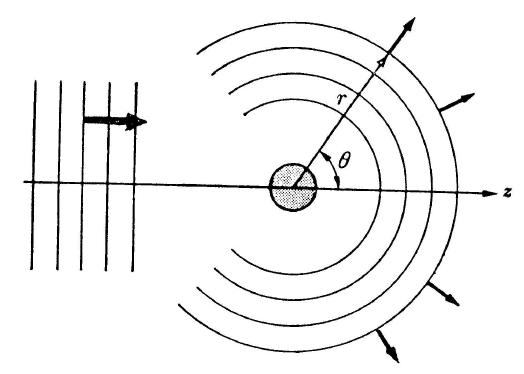
\includegraphics[height=1.29in,width=1.91in,viewport=0 0 400 275,clip]{Figures/Pseudo-scatter.jpg}
\caption{\fontsize{5.5pt}{4.2pt}\selectfont{\textrm{Schematic illustration of electromagnetic wave propagation.}}}%(与文献\cite{EPJB33-47_2003}图1对比)
\label{Light-Wave}
\end{figure}
}

\frame{
	\frametitle{固体光学常数间的基本关系}
	\begin{itemize}
		\item 角频率为$\omega$的电磁波(横波)在均匀介质中传播(设为$x$方向)
			\begin{displaymath}
				\mathbf{E}(\vec r,t)=E(z)\mathrm{e}^{-\mathrm{i}\omega t}(0,0,1)\qquad\mathbf{E}\perp x
			\end{displaymath}
			根据\textrm{Maxwell~}方程,可有电场与电流密度的基本关系
			\begin{displaymath}
				\frac{\mathrm{d}^2E(z)}{\mathrm{d}z^2}=-\frac{\omega^2}{c^2}E(z)-\frac{4\pi\mathrm{i}\omega}{c^2}J(z)
			\end{displaymath}
		\item 引入复数电导率$\sigma(\sigma)=\sigma_1(\omega)+\mathrm{i}\sigma_2(\omega)$
			\begin{displaymath}
				J(z)=\sigma(\omega)E(z)=\sigma_1(\omega)E(z)+\mathrm{i}\sigma_2(\omega)E(z)
			\end{displaymath}
			吸收介质中电流$\mathbf{j}$分为两部分,一部分与$\mathbf{E}$相位差$90^{\circ}$,称为\textcolor{magenta}{极化电流},一部分与电场$\mathbf{E}$同相位,称为\textcolor{magenta}{传导电流}\\
			\textcolor{red}{注意}:~极化电流与电场相位差$90^{\circ}$,在一个周期平均电场做工为零,不消耗电磁场能量
	\end{itemize}
}

\frame
{
	\frametitle{固体光学常数间的基本关系}
	\begin{itemize}
		\item 当载流子迁移距离比电磁波的波长小得多时(长波极限),可忽略电磁波在空间变化的影响
			\begin{displaymath}
				\frac{\mathrm{d}^2E(z)}{\mathrm{d}z^2}=-\frac{\omega^2}{c^2}\left[ 1+\frac{4\pi\mathrm{i}\omega\sigma(\omega)}{\omega} \right]E(z)
			\end{displaymath}
		可解得电磁波在介质内的衰减
		\begin{displaymath}
			E(z)=E_0\mathrm{e}^{\mathrm{i}(\omega/c)Nz}
		\end{displaymath}
		这里$N$是复数折射率,满足
		\begin{displaymath}
			N^2=1+\frac{4\pi\mathrm{i}\sigma(\omega)}{\omega} 
		\end{displaymath}
		\item 复数折射写成$N=n+\mathrm{i}k$,其中$n$是折射指数,$k$是消光系数,因此
			\begin{displaymath}
				E(z)=E_0\mathrm{e}^{\mathrm{i}(\omega/c)nz}\mathrm{e}^{-(\omega/c)kz}
			\end{displaymath}
			因此电磁波在介质中传播速度$c/n$,透射深度$\delta(\omega)=\frac{c}{\omega k(\omega)}$
	\end{itemize}
}

\frame
{
	\frametitle{固体光学常数间的基本关系}
	\begin{itemize}
		\item 吸收系数
			\begin{displaymath}
				\alpha(\omega)=\frac{2\omega k(\omega)}c\equiv\frac2{\delta(\omega)}
			\end{displaymath}
		\item 电磁波在介质中传播,根据介电函数和复数折射率的关系$N^2=\varepsilon$,因此
			\begin{displaymath}
				\varepsilon_1=n^2-k^2\qquad\varepsilon_2=2nk
			\end{displaymath}
			相应地
			\begin{displaymath}
				n^2=\frac12(\varepsilon_1+\sqrt{\varepsilon_1^2+\varepsilon_2^2})\quad k^2=\frac12(-\varepsilon_1+\sqrt{\varepsilon_1^2+\varepsilon_2^2})
			\end{displaymath}
			根据等式$\varepsilon(\omega)=1+\dfrac{4\pi\mathrm{i}\sigma(\omega)}{\omega}$有
			\begin{displaymath}
				\varepsilon_1=1-\frac{4\pi\sigma_2(\omega)}{\omega}\qquad\varepsilon_2=\frac{4\pi\sigma_1(\omega)}{\omega} 
			\end{displaymath}
			\textcolor{red}{注意}:~\textcolor{blue}{确定介电函数虚部与电导率实部间的关系}
	\end{itemize}
}

\frame
{
	\frametitle{固体光学常数间的基本关系}
	\begin{itemize}
		\item 电磁波垂直入射时,反射波与入射波分别为
\begin{figure}[h!]
\centering
%\hspace*{-10pt}
\vspace*{-0.4in}
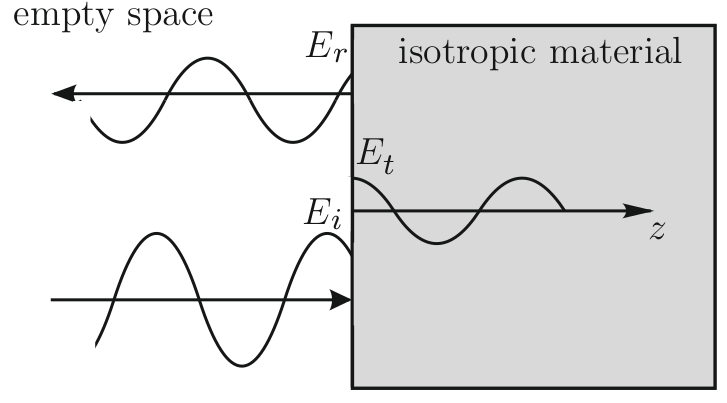
\includegraphics[height=1.2in,width=1.8in,viewport=0 0 750 600,clip]{Figures/Optic-reflect.png}
\caption{\fontsize{5.5pt}{4.2pt}\selectfont{\textrm{Schematic representation of incident, reflected and transmitted electromagnetic\\ wave at the surface.}}}%
\label{Optic-reflect}
\end{figure} 
			\begin{displaymath}
				\begin{aligned}
					&E(z)=E_t\mathrm{e}^{\mathrm{i}(\omega/c)Nz}\quad z>0\\
					&E(z)=E_i\mathrm{e}^{\mathrm{i}(\omega/c)z}+E_r\mathrm{e}^{-\mathrm{i}(\omega/c)z}\quad z<0\\
				\end{aligned}
			\end{displaymath}
			反射率$R$可以表示为
			\begin{displaymath}
				R=\left|\frac{E_r}{E_i}\right|^2=\left|\frac{1-N}{1+N}\right|^2=\frac{(n-1)^2+k^2}{(n+1)^2+k^2}
			\end{displaymath}
	\end{itemize}
}

\subsection{载流子与\rm{Lorentz-Drude}模型}
%\subsection{光子与电子的激发}
\frame
{
	\frametitle{光子与电子的激发}
	电磁波在介质中的传播,伴随了光子与介质中电子的相互作用
\begin{figure}[h!]
\centering
\vspace*{-10pt}
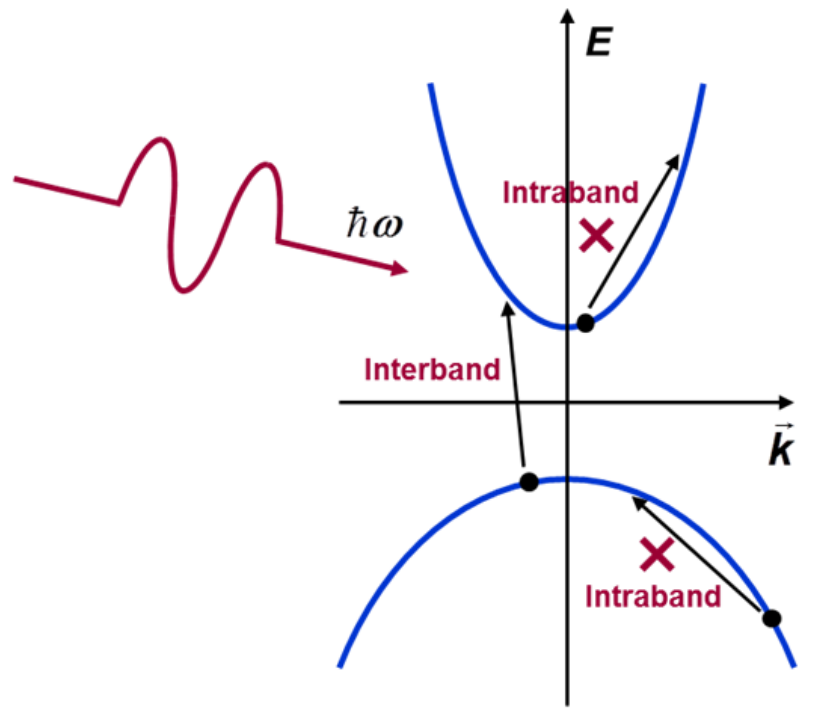
\includegraphics[height=2.3in,width=2.2in,viewport=0 0 800 800,clip]{Figures/Inter-Intra_band-transition.png}
\caption{\fontsize{5.5pt}{4.2pt}\selectfont{\textrm{Schematic representation of interaction of photons and the electrons in the semiconductor.}}}%
\label{Optic-transition}
\end{figure} 
}

\frame
{
	\frametitle{光子与电子的激发}
	粒子间相互作用遵守能量守恒与动量守恒:~\\
	假设介质中的电子初始态为$\vec k_i$,对应的能量为$E_n(\vec k_i)$,电子吸收入射光子跃迁到终态$\vec k_f$,能量变为$E_m(\vec k_f)$,则有
	\begin{itemize}
		\item \textcolor{blue}{能量守恒}
			\begin{displaymath}
				E_m(\vec k_f)=E_n(\vec k_i)+\hbar\omega
			\end{displaymath}
			$\hbar\omega$是入射光子能量
		\item \textcolor{blue}{动量守恒}
			\begin{displaymath}
				\vec k_f=\vec k_i+\vec q
			\end{displaymath}
			$\vec q$是入射光子的动量
	\end{itemize}
	具体计算过程中,考虑光子引起的介质中电子的状态变化,采取了一系列的简化
}

\frame
{
	\frametitle{电场中的自由电子:~\textrm{Lorentz}模型}
	\begin{itemize}
		\item 载流子在外电场$\mathbf{E}(\vec r,t)=\mathbf{E}_0\mathrm{e}^{\mathrm{i}(\vec q\cdot\vec r-\omega t)}$下的运动方程
			\begin{displaymath}
				m\ddot{\vec r}=-\frac m{\tau}\dot{\vec r}+(-e)\mathbf{E}_0\mathrm{e}^{\mathrm{i}(\vec q\cdot\vec r-\omega t)}
			\end{displaymath}
			这里$\vec r(t)$是载流子坐标,$\tau$是\textcolor{red}{唯象弛豫时间}
		\item 长波极限下,忽略电磁波在空间的变化
			\begin{displaymath}
				m\ddot{\vec r}=-\frac m{\tau}\dot{\vec r}-e\mathbf{E}_0\mathrm{e}^{-\mathrm{i}\omega t}
			\end{displaymath}
			取载流子位置函数$\vec r(t)=\vec A_0\mathrm{e}^{-\mathrm{i}\omega t}$,有
			\begin{displaymath}
				\vec A_0=\frac{e\tau}m\frac1{(\omega^2+\mathrm{i}\omega\tau-\omega_0^2)}\mathbf{E}_0
			\end{displaymath}
	\end{itemize}
	经典图像中,介质中载流子的运动可类比于谐振子,$\omega_0$为弹簧的固有频率
}

%\frame
%{
%	\frametitle{\textrm{Lorentz}模型}
%由谐振子偶极与电场的关系(电极化率)可有
%\begin{displaymath}
%\begin{aligned}
%	\mathbf{P}=&N\mathbf{p}\\
%	\mathbf{P}=&\varepsilon_0\chi_{\mathrm{e}}\mathbf{E}\\
%	\varepsilon=&1+\chi_{\mathrm{e}}
%\end{aligned}
%\end{displaymath}
%这里$\chi_{\mathrm{e}}$称为电极化率
%\begin{displaymath}
%\begin{aligned}
%	\vec p=&q\vec r(t)\\
%	=&\dfrac{q^2}m\dfrac1{(\omega^2+\mathrm{i}\omega\tau-\omega_0^2)}\mathbf{E}_0\mathrm{e}^{-\mathrm{i}\omega t}\\
%	=&\dfrac{q^2}m\dfrac1{(\omega^2+\mathrm{i}\omega\tau-\omega_0^2)}\mathbf{E}
%\end{aligned}
%\end{displaymath}
%因此
%\begin{displaymath}
%	\varepsilon=1+\dfrac{Nq^2}{m\varepsilon_0}\dfrac1{(\omega^2+\mathrm{i}\omega\tau-\omega_0^2)}\Longrightarrow \omega_{\mathrm{p}}^2=\dfrac{Nq^2}{m\varepsilon_0}	
%\end{displaymath}
%}
%
\frame
{
	\frametitle{\textrm{Lorentz}模型}
\begin{figure}[h!]
\centering
\vspace*{-5pt}
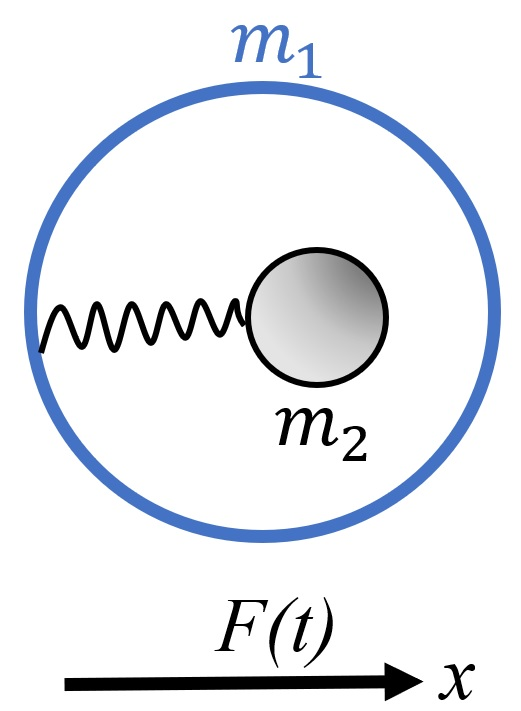
\includegraphics[height=1.05in,width=0.7in,viewport=0 0 380 550,clip]{Figures/A_mechanical_model_giving_rise_to_the_negative_effective_mass_effect.jpg}
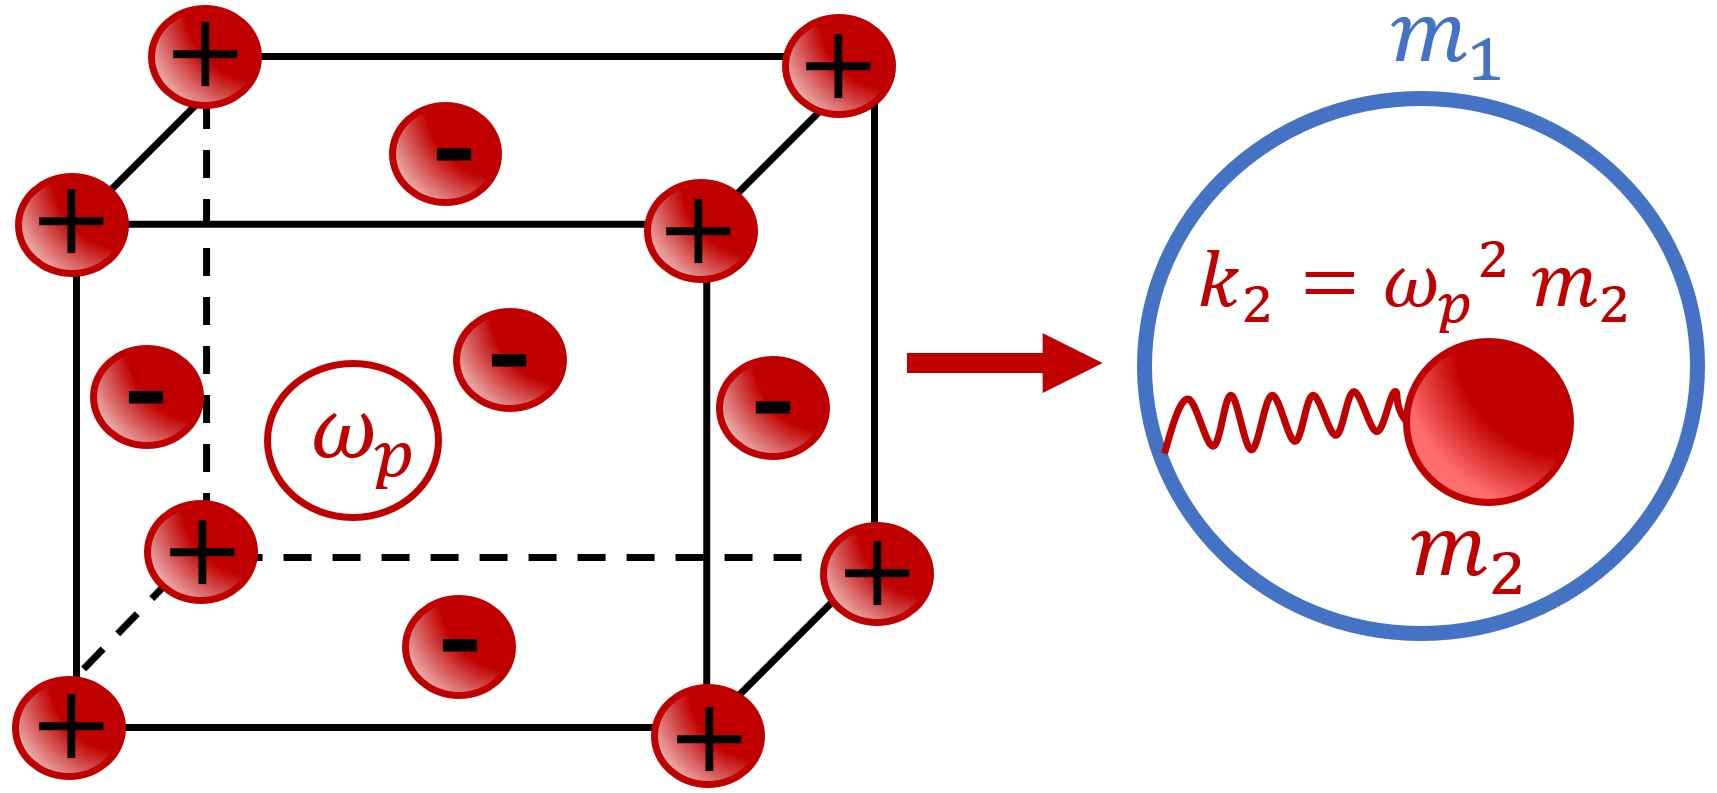
\includegraphics[height=1.55in,width=3.25in,viewport=0 0 1300 600,clip]{Figures/Equivalent_mechanical_scheme_of_electron_gas_in_ionic_lattice.jpg}
\caption{\fontsize{5.5pt}{4.2pt}\selectfont{\textrm{Equivalent mechanical scheme of electron gas in ionic lattice.}}}%
\label{Electron-gas-in-lattice}
\end{figure} 
			$\omega_{\mathrm{p}}$是载流子的等离振荡频率
			\begin{displaymath}
				\omega_{\mathrm{p}}^2=\frac{4\pi ne^2}m
			\end{displaymath}
}

\frame
{
	\frametitle{电场对导带电子的影响}
\begin{figure}[h!]
\centering
\vspace*{-13pt}
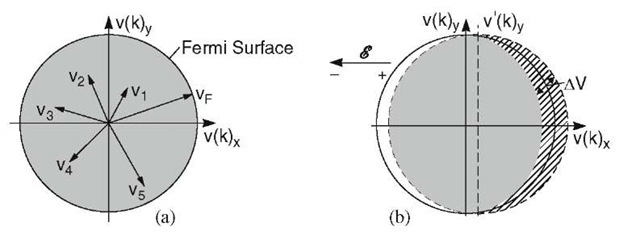
\includegraphics[height=1.4in,width=3.8in,viewport=0 0 480 180,clip]{Figures/Electrmagnetic_Fermi-surface-1.jpg}
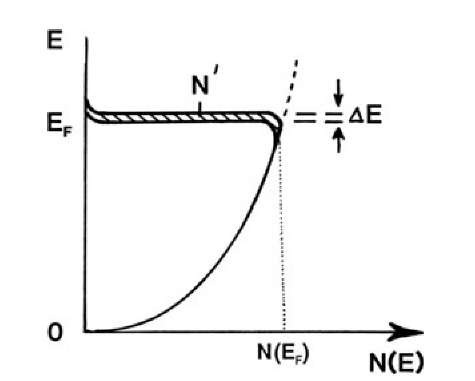
\includegraphics[height=1.35in,width=2.2in,viewport=0 0 200 130,clip]{Figures/Electrmagnetic_Fermi-surface-2.jpg}
\caption{\fontsize{5.5pt}{4.2pt}\selectfont{\textrm{Schematic representation of the Fermi-surface affected by the electrmagnetic field.}}}%
\label{CB-Electron-in-E}
\end{figure} 
}

\frame
{
	\frametitle{\textrm{Lorentz-Drude}模型}
\begin{itemize}
	\item \textrm{Lorentz-Model}:\\
		始于电子与晶格离子间作用,侧重描述电子在固体中的运动,介电函数为
		\begin{displaymath}
			\varepsilon(\omega)=1-\dfrac{\omega_{\mathrm{p}^2}}{\omega^2+\mathrm{i}\omega\tau-\omega_0^2}
		\end{displaymath}
		\textcolor{blue}{\textrm{Lorentz}模型中,取$\omega_0=0$,即为\textrm{Drude}模型}
	\item \textrm{Drude-Model}:\\
		侧重描述自由电子气对外部交变电场的响应,则介电函数可以表示为:
			\begin{displaymath}
				\varepsilon(\omega)=1-\frac{\omega_\mathrm{p}^2}{\omega(\omega+\mathrm{i}/\tau)}=\underline{\textcolor{blue}{\left[ 1-\frac{\omega_{\mathrm{p}}^2\tau^2}{1+\omega^2\tau^2} \right]}}+\mathrm{i}\underline{\textcolor{blue}{\left[ \frac{\omega_{\mathrm{p}}^2\tau}{\omega(1+\omega^2\tau^2)} \right]}}
			\end{displaymath}
%\begin{displaymath}
\end{itemize}
}

\frame
{
	\frametitle{\textrm{Lorentz-Drude}模型}
\begin{figure}[h!]
\centering
\vspace*{-13pt}
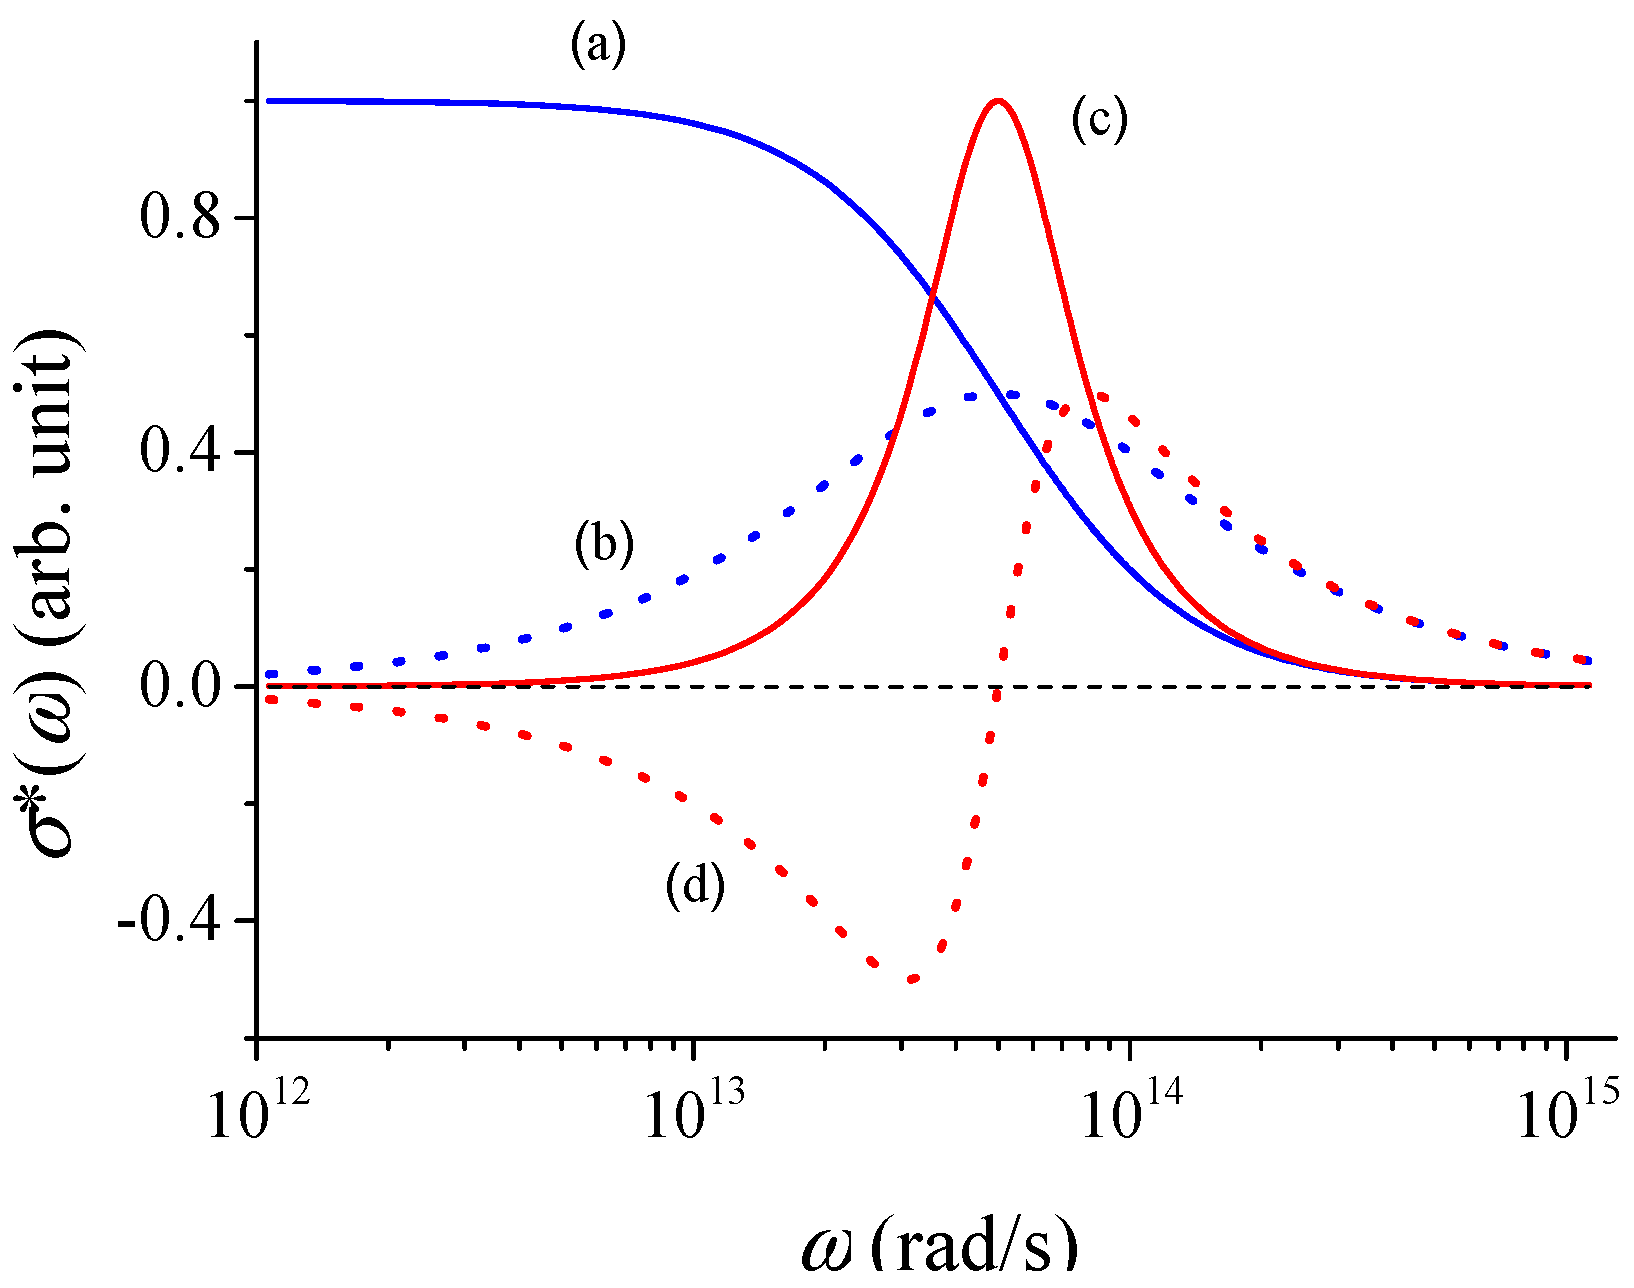
\includegraphics[height=2.5in,width=3.6in,viewport=0 0 200 155,clip]{Figures/Optical-conductivity-in-the-Drude-relaxation-and-in-the-Lorentz-resonance.png}
\caption{\fontsize{5.5pt}{4.2pt}\selectfont{\textrm{Optical conductivity in the Drude relaxation ((a) and (b)) and in the Lorentz resonance ((c) and (d)).}}}%
\label{Drude-vs-Lorentz}
\end{figure} 
}

\frame
{
	\frametitle{\textrm{Lorentz-Drude}模型}
\begin{figure}[h!]
\centering
\vspace*{-13pt}
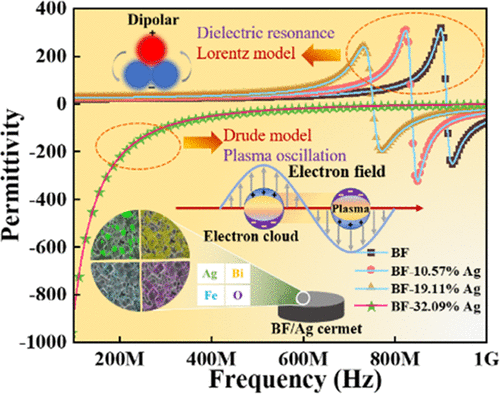
\includegraphics[height=2.7in,width=3.6in,viewport=0 0 500 400,clip]{Figures/Lorentz_Drude-model.png}
\caption{\fontsize{5.5pt}{4.2pt}\selectfont{\textrm{Optical permittivity in the Plasma oscillation and in the Dielectric resonance.}}}%
\label{Drude-vs-Lorentz}
\end{figure} 
}

\frame
{
	\frametitle{\textrm{Drude}模型}
	\textcolor{blue}{在远红外区,经典自由电子气模型可以很好地描述金属的光学行为}
	如果载流子密度为$n$,则电流密度
	\begin{displaymath}
		\mathbf{J}=n(-e)\dot{\vec r}=n(-e)(-\mathrm{i}\omega)\vec A_0\mathrm{e}^{-\mathrm{i}\omega t}=\frac{ne^2\tau}m\frac1{1-\mathrm{i}\omega\tau}\mathbf{E}_0\mathrm{e}^{-\mathrm{i}\omega t}
	\end{displaymath}
	由此可得频率有关的电导率表示为
	\begin{displaymath}
		\sigma(\omega)=\frac{ne^2\tau}m\frac1{1-\mathrm{i}\omega\tau}=\sigma_0\frac1{1-\mathrm{i}\omega\tau}
	\end{displaymath}
	其中$\sigma_0=ne^2\tau/m$是静态电导率
%	\begin{itemize}
%		\item 
	介电函数可表示为
	\begin{displaymath}
	\epsilon_1(\omega)=1-\frac{\omega_{\mathrm{p}}^2\tau^2}{1+\omega^2\tau^2}\quad \epsilon_2(\omega)=\frac{\omega_{\mathrm{p}}^2\tau}{\omega(1+\omega^2\tau^2)}\quad
\end{displaymath}
%	\end{itemize}
}

\subsection{带间电子的激发}
\frame
{
\frametitle{带间跃迁的计算}
\begin{itemize}
\setlength{\itemsep}{10pt}
	\item 用半经典方法处理周期性体系的光学性质,用量子力学处理介质,对电磁波仍然采用经典电动力学描写
	\item 以半导体中的带间垂直跃迁(价带$|v,\vec k\rangle$,导带$|c,\vec k\rangle$)为例讨论固体的能带间跃迁(\textcolor{red}{含时微扰})
\begin{figure}[h!]
\centering
%\hspace*{-10pt}
\vspace*{-0.2in}
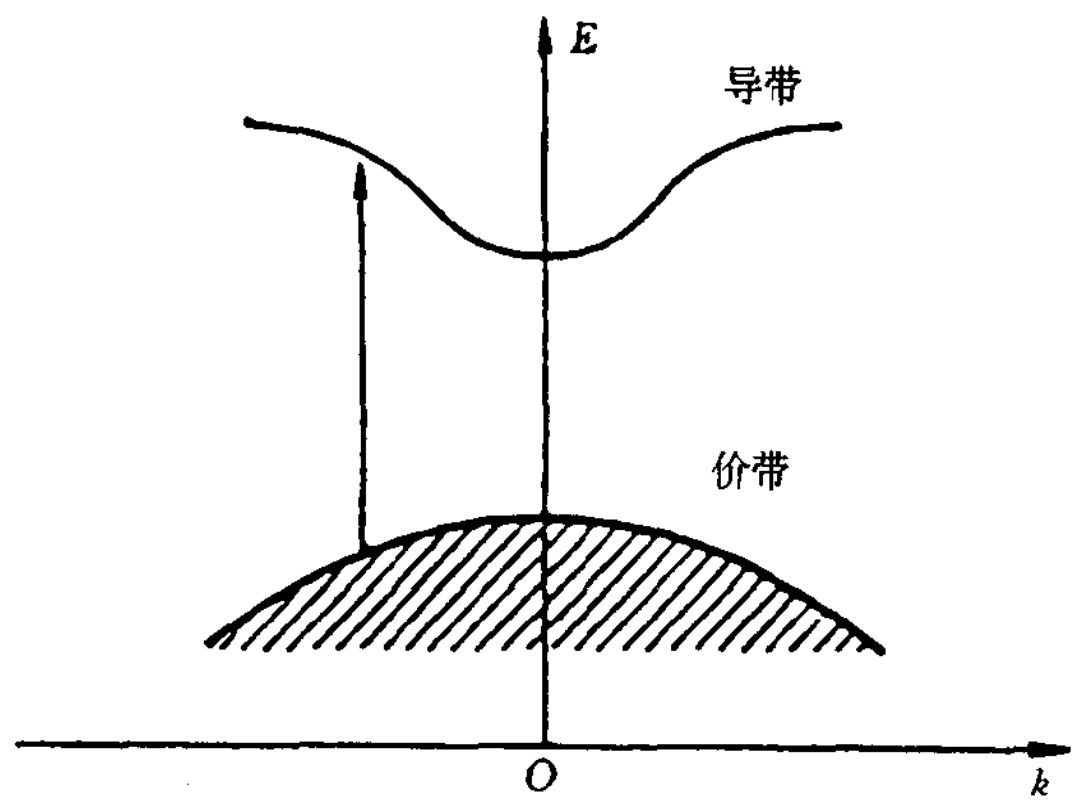
\includegraphics[height=1.8in,width=2.0in,viewport=0 0 1000 900,clip]{Figures/optic_dir.png}
\caption{\fontsize{8.0pt}{5.2pt}\selectfont\textrm{Schematic representation of directly inter-band transition.}}%
\label{Optic-dir}
\end{figure} 
\end{itemize}
}

\frame
{
	\frametitle{\textrm{Lorenz~gauge}}
	根据\textrm{Lorenz}规范\footnote{\fontsize{5.2pt}{4.0pt}\selectfont{\textrm{Lorenz}在1867年提出的电磁势满足的规范条件:~
	\begin{displaymath}
		\nabla\cdot\mathbf{A}+\mu_0\varepsilon_0\frac{\partial\phi}{\partial t}=0
	\end{displaymath}
	\textcolor{red}{注}:~\textrm{Ludvig Valentin Lorenz~(1829-1891)}是丹麦人(中译作~\textcolor{blue}{洛伦茨})\\
  	~~~~~\textrm{Hendrik A. Lorentz~(1853-1928)是荷兰人(中译作~\textcolor{blue}{洛伦兹})}}},电磁场可以表示为
\begin{displaymath}
%  \left\{
\begin{aligned}
	\vec E&=-\nabla\phi-\frac{\partial\mathbf{A}}{\partial t}\\
	\vec B&=\nabla\times\mathbf{A}
  \end{aligned}%\right. 
  \label{eq:optic-26}
\end{displaymath}
%\end{itemize}
{\fontsize{8.2pt}{4.0pt}\selectfont{式中$\phi$为是标量势,$\mathbf{A}$是矢量势}}\\
%\begin{itemize}
%频率为$\omega$的平面偏振光,
当电子体系用单电子\textrm{Hamiltonian}描述时
\begin{displaymath}
	H_0=\frac{{\vec p}^2}{2m}+V(\vec r)
\end{displaymath}
辐射场$\mathbf{A}$与电子的作用会引起电子动量的改变,应用含时微扰理论,电子的动量将表示为
	\begin{displaymath}
		\mathbf{p}\rightarrow\vec p+\frac{e}{c}\mathbf{A}(\vec r,t)
	\end{displaymath}
%	{\fontsize{7.2pt}{4.0pt}\selectfont{这里$e$是电子电荷,$c$是光速}}
}

\frame
{
	\frametitle{横波电磁场下的电场与电子的相互作用}
	当\textcolor{blue}{标量势为零}($\phi=0$),并且矢量势满足~\textcolor{purple}{\textrm{Coulomb}规范}
	\begin{displaymath}
		\nabla\cdot\mathbf{A}=0
	\end{displaymath}
	因此\textcolor{blue}{标量积$\mathbf{p}\cdot\mathbf{A}$与$\mathbf{A}\cdot\mathbf{p}$相等},有
\begin{displaymath}
	\hspace*{-10pt}
	H=\frac1{2m}[\vec p+\frac{e}c\mathbf{A}(\vec r,t)]^2+V(\vec r)=\left[ \frac{\vec p^2}{2m}+V(\vec r) \right]+\textcolor{blue}{\frac{e}{mc}\mathbf{A}\cdot\vec p}+\textcolor{magenta}{\frac{e^2}{2mc^2}\mathbf{A}^2}
\end{displaymath}
其中后两项表示量子尺度内电子与矢量场的相互作用,并忽略电子自旋与磁场的相互作用

\textcolor{blue}{频率为$\omega$的横波},波矢为$\vec q$,电场极化矢量方向$\mathbf{e}$,则矢量势
\begin{displaymath}
	\mathbf{A}(\vec r,t)=A_0\mathbf{e}\mathrm{e}^{\mathrm{i}(\vec q\cdot\vec r-\omega t)}+\mathrm{c.c}\quad\textcolor{red}{\mathbf{e}\bot\vec q}
\end{displaymath}
准确到$\mathrm{A}$的线性项(忽略$\mathrm{A}$的平方项)\footnote{\fontsize{5.2pt}{4.0pt}\selectfont{偶极近似下,这是合理的近似}},则体系~\textrm{Hamiltonian}为:
\begin{displaymath}
	H=\left[ \frac{\vec p^2}{2m}+V(\vec r) \right]+\frac{eA_0}{mc}\mathrm{e}^{\mathrm{i}(\vec q\cdot\vec r-\omega t)}\mathbf{e}\cdot\vec p+\frac{eA_0}{mc}\mathrm{e}^{-\mathrm{i}(\vec q\cdot\vec r-\omega t)}\mathbf{e}\cdot\vec p
\end{displaymath}
%	\item 
}

\frame
{
\frametitle{带间跃迁与电导}
在含时微扰\textrm{Hamiltonian}作用下,带间跃迁的能量贡献为
\begin{displaymath}
	\begin{aligned}
		W(\vec q,\omega)=&\frac{2\pi}{\hbar}\left( \frac{eA_0}{m_ec} \right)^2\textcolor{blue}{2}\sum_{i,j}|\langle\psi_j|\mathrm{e}^{\mathrm{i}\vec q\cdot\vec r}\mathbf{e}\cdot\vec p|\psi_i\rangle|^2\\
		\times&\delta[E_j-E_i-\hbar\omega][f(E_i)-f(E_j))]
	\end{aligned}
  \label{eq:optic-27}
\end{displaymath}
\begin{itemize}
	\item $\delta$因子表示跃迁过程的能量守恒关系
	\item 系数\textcolor{blue}{$2$}表示自旋简并态求和
\end{itemize}
%矩阵元$\langle c\vec k|H'|v\vec k\rangle$表示\textrm{Bloch}函数间的积分
忽略磁场贡献,%矩阵元可以简写成$\dfrac1cA_0\vec e\cdot\vec M_{cv}(\vec k)$,$\vec s$为电磁波矢量势$\vec A_0(=A_0\vec s)$方向的单位矢量。
只有满足能量守恒和动量守恒条件的跃迁才对积分有贡献。%$\displaystyle\int W\dfrac{\textrm{d}\vec k}{(2\pi)^3}$为单位体积、单位时间内吸收能量为$\omega$的光子的总数,系数2是考虑两种自旋态。将式\eqref{eq:optic-27},\eqref{eq:optic-28}代入式\eqref{eq:optic-29},并应用$\dfrac{A_0}c\vec e\cdot\vec M_{cv}(\vec k)$表示矩阵元,得

在介质中由矢量势产生的电场为
\begin{displaymath}
	\textcolor{red}{\mathbf{E}(\vec r,t)=-\frac1c\frac{\partial\mathbf{A}}{\partial t}}=E_0\mathbf{e}\mathrm{e}^{\mathrm{i}\vec q\cdot\vec r-\omega t}+\mathrm{c.c}\quad\mbox{其中}E_0=\mathrm{i}\omega\frac{A_0}c
\end{displaymath}

介质中的传导电流(与电场方向平行)
\begin{displaymath}
	\mathbf{J}(\vec r,t)=\sigma(\vec q,\omega)E_0\mathbf{e}\mathrm{e}^{\mathrm{i}(\vec q\cdot\vec r-\omega t)}+\mathrm{c.c}\quad(\textcolor{red}{\mathbf{e}\bot\vec q})
\end{displaymath}
}

\frame
{
	\frametitle{横向介电函数\textrm{(transverse dielectric function)}}
	当存在外电场$\mathbf{E}$,介质中的传导电流$\mathbf{J}$单位时间消耗的能量为$\int_V\mathbf{J}\cdot\mathbf{E}\mathrm{d}\vec r$,因此有
由此计算得到吸收功率
{\fontsize{8.2pt}{6.2pt}\selectfont{
\begin{displaymath}
	\begin{aligned}
		\int_V\mathbf{J}\cdot\mathbf{E}\mathrm{d}\vec r=&\int_V[\sigma(\vec q,\omega)E_0\mathrm{e}^{\vec q\cdot\vec r-\omega t}+\mathrm{c.c}][E_0\mathrm{e}^{\vec q\cdot\vec r-\omega t}+\mathrm{c.c}]\mathrm{d}\vec r=\sigma(\vec q,\omega)|E_0|^2V+\mathrm{c.c}\\
		=&2\sigma_{\textcolor{blue}{1}}(\vec q,\omega)|E_0|^2V=2\sigma_1(\vec q,\omega)\frac1{c^2}\omega^2A_0^2V=\textcolor{blue}{\hbar\omega W(\vec q,\omega)}
	\end{aligned}
\end{displaymath}}}
因此电导率的实部为
\begin{displaymath}
	\sigma_1(\vec q,\omega)=\frac{e^2}{2V}\frac{\hbar\omega W(\vec q,\omega)}{\omega^2A_0^2}
\end{displaymath}
根据介电函数与电导率的关系,有
\begin{displaymath}
	\varepsilon(\vec q,\omega)=1+\frac{4\pi\mathrm{i}}{\omega}\sigma(\vec q,\omega)
\end{displaymath}
于是横向介电函数的虚部为
\begin{displaymath}
	\varepsilon_2(\vec q,\omega)=\frac{8\pi^2e^2}{m_e^2\omega^2}\frac1V\sum_{ij}|\langle\psi_j|\mathrm{e}^{\mathrm{i}\vec q\cdot\vec r}\mathbf{e}\cdot\vec p|\psi_i\rangle|^2\delta(E_j-E_i-\hbar\omega)[f(E_i)-f(E_j)]
\end{displaymath}
}

\frame
{
	\frametitle{$\vec k$空间表示的横向介电函数}
对于周期体系,横向介电函数的虚部为
{\fontsize{9.2pt}{6.2pt}\selectfont{
\begin{displaymath}
	\hspace*{-13pt}
	\varepsilon_2(\vec q,\omega)=\frac{8\pi^2e^2}{m_e^2\omega^2}\frac1V\sum_{i,j,\vec k}|\langle\psi_{\vec k+\vec q}^c|\mathrm{e}^{\mathrm{i}\vec q\cdot\vec r}\mathbf{e}\cdot\vec p|\psi_{\vec k}^v\rangle|^2\delta(E_{\vec k+\vec q}^c-E_{\vec k}^v-\hbar\omega)[f(E_{\vec k}^v)-f(E_{\vec k+\vec q}^c)]
\end{displaymath}}}
{\fontsize{7.5pt}{6.2pt}\selectfont{
\textrm{Block}表象下,波函数$|\psi_{\vec k}^n\rangle=\mathrm{e}^{\mathrm{i}\vec k\cdot\vec r}|u_{\vec k}^n\rangle$的周期部分$|u_{\vec k}^n\rangle$对应的\textrm{Hamiltonian}写成
\begin{displaymath}
	H_0(\vec k)=-\frac{\hbar^2}{2m_e}(\vec p_{\vec k})^2+V = -\frac{\hbar^2}{2m_e}(\nabla+\mathrm{i}\vec k)^2+V
\end{displaymath}
并有$H_0(\vec k)|u_{\vec k}^n\rangle=E_{\vec k}^n|u_{\vec k}^n\rangle$\\
注意到关系式
	\begin{displaymath}
		\begin{aligned}
			&\dfrac{\partial H(\vec k)}{\partial \vec k}=\mathrm{i}[H_{\vec k},\vec r]=\hbar\vec v_k=\hbar\frac{\vec p_k}{m_e}=-\mathrm{i}\frac{\hbar^2}{m_e}(\nabla+\mathrm{i}\vec k)\\
			&\Longrightarrow\langle u_{m\vec k}|[\vec r,H_{\vec k}]|u_{n\vec k}\rangle=(E_{n\vec k}-E_{m\vec k})\langle u_{m\vec k}|\vec r|u_{n\vec k}\rangle
		\end{aligned}
	\end{displaymath}
}}
在$\vec k$空间,横向介电函数的虚部可表示为
{\fontsize{6.5pt}{6.2pt}\selectfont{
\begin{displaymath}
	\hspace*{-10pt}
	\varepsilon_2(\vec q,\omega)=\frac{8\pi^2e^2}{\omega^2}\frac1V\sum_{i,j,\vec k}|\langle u_{\vec k+\vec q}^c|\mathrm{e}^{\mathrm{i}\vec q\cdot\vec r}\mathbf{e}\cdot\vec r|u_{\vec k}^v\rangle(E_{\vec k+\vec q}^c-E_{\vec k}^v)|^2\delta(E_{\vec k+\vec q}^c-E_{\vec k}^v-\hbar\omega)[f(E_{\vec k}^v)-f(E_{\vec k+\vec q}^c)]
\end{displaymath}}}
当$\vec q$足够小时,可引入假设$\psi_{\vec k+\vec q}^c\approx\mathrm{exp}(\mathrm{i}\vec q\cdot\vec r)\psi_{\vec k}^c$,%于是可有
%{\fontsize{9.5pt}{6.2pt}\selectfont{
%\begin{displaymath}
%	\hspace*{-15pt}
%	\varepsilon_2(\omega)\approx\frac{8\pi^2e^2}{m_e^2\omega^2}\frac1V\sum_{i,j,\vec k}|\langle u_{\vec k}^c|\mathbf{e}\cdot(\mathrm{i}\nabla-\vec k)|u_{\vec k}^v\rangle|^2\delta(E_{\vec k}^c-E_{\vec k}^v-\hbar\omega)[f(E_{\vec k}^v)-f(E_{\vec k}^c)]
%\end{displaymath}}}
简化计算
}

\frame
{
	\frametitle{长波极限下的横向介电函数}
因此,在长波极限下($\vec q\rightarrow0$),横向介电函数虚部简化为
\begin{displaymath}
	\begin{aligned}
		\varepsilon_2(\omega)=&\lim_{\vec q\rightarrow0}\frac{8\pi^2e^2}{m_e^2\omega^2}\sum_{v}^{\mathrm{occ}}\sum_{c}^{\mathrm{unocc}}\int\frac{\mathrm{d}\vec k}{(2\pi)^3}|\langle c,\vec k|\mathbf{e}\cdot\vec p|v,\vec k\rangle|^2\\
		\times&\delta(E_c(\vec k)-E_v(\vec k)-\hbar\omega)[f(E_c(\vec k))-f(E_v(\vec k))]
	\end{aligned}
  \label{eq:optic-varepsilon_2}
\end{displaymath}
$\varepsilon_2(\omega)$是晶体的光学吸收和能带结构之间的基本关系

对应的$\varepsilon_1$可以根据\textrm{Kramers-Kr\"onig}关系%\eqref{eq:optic-16}
得到
\begin{displaymath}
	\varepsilon_1(\omega)=1+\frac1{\pi}\mathscr{P}\int_{-\infty}^{+\infty}\frac{\varepsilon_2(\omega^{\prime})}{\omega^{\prime}-\omega}\textrm{d}\omega^{\prime}=1+\frac2{\pi}\mathscr{P}\int_0^{+\infty}\frac{\omega^{\prime}\varepsilon_2(\omega^{\prime})}{\omega^{\prime2}-\omega^2}\textrm{d}\omega^{\prime}
  \label{eq:optic-varepsilon_1}
\end{displaymath}
因此介电函数表示为
{\fontsize{9.5pt}{6.2pt}\selectfont{
\begin{displaymath}
	\hspace*{-13pt}
	\varepsilon(\omega)=1+\frac{8\pi e^2}{m_e^2}\sum_{v,c}\int\frac{\mathrm{d}\vec k}{(2\pi)^3}\frac{|\langle c,\vec k|\mathbf{e}\cdot\vec p|v,\vec k\rangle|^2}{(E_c(\vec k)-E_v(\vec k))^2/\hbar^2}\frac{[f(E_v(\vec k))-f(E_c(\vec k))]}{E_c(\vec k)-E_v(\vec k)-\hbar\omega-\mathrm{i}\eta}
  \label{eq:optic-varepsilon}
\end{displaymath}}}
}

\frame
{
	\frametitle{带内跃迁$^{\ast}$}
\fontsize{8.2pt}{6.2pt}\selectfont{
一般地,带内跃迁的电导率函数可表示为
\begin{displaymath}
	\sigma(\vec q,\omega)=\frac{2e^2}{m_e^2}\int\frac{\mathrm{d}\vec k}{(2\pi)^3}\frac{|\langle\psi_{\textcolor{red}{\vec k+\vec q}}|\mathrm{e}^{\mathrm{i}\vec q\cdot\vec r}\mathbf{e}\cdot\vec p|\psi_{\textcolor{red}{\vec k}}\rangle|^2}{(E_{\textcolor{red}{\vec k+\vec q}}-E_{\textcolor{red}{\vec k}})/\hbar}\frac{(-\mathrm{i})[f(E_{\textcolor{red}{\vec k}})-f(E_{\textcolor{red}{\vec k+\vec q}})]}{E_{\textcolor{red}{\vec k+\vec q}}-E_{\textcolor{red}{\vec k}}-\hbar\omega-\mathrm{i}\eta}
  \label{eq:optic-intra-sigma}
\end{displaymath}
%\textcolor{violet}{推广到长波极限下的带内跃迁}
当$\vec q$足够小,有近似
\begin{displaymath}
	f(E_{\vec k+\vec q})-f(E_{\vec k})\approx\frac{\partial f}{\partial E}(E_{\vec k+\vec q}-E_{\vec k})
\end{displaymath}
\textcolor{violet}{假设$\psi_{\vec k+\vec q}\approx\mathrm{exp}(\mathrm{i}\vec q\cdot\vec r)\psi_{\vec k}$成立},于是可有
\begin{displaymath}
	\frac1{m_e}\langle\psi_{\vec k+\vec q}|\mathrm{e}^{\mathrm{i}\vec q\cdot\vec r}\vec p|\psi_{\vec k}\rangle\approx\frac1{m_e}\langle\psi_{\vec k}|\vec p|\psi_{\vec k}\rangle=\vec v
\end{displaymath}
\begin{displaymath}
	\sigma(\vec q,\omega)=\frac{e^2\hbar}{4\pi^3}\int\mathrm{d}\vec k(\mathbf{e}\cdot\vec v)^2\frac{-\mathrm{i}}{E_{\vec k+\vec q}-E_{\vec k}-\hbar\omega-\mathrm{i}\eta}\left(\textcolor{red}{ -\frac{\partial f}{\partial E}} \right)
\end{displaymath}
注意到%$E_{\mathrm{\vec k+\vec q}}-E_{\mathrm{k}}\approx\vec q\cdot(\partial E/\partial\vec k)=\vec q\cdot\vec v\hbar$,:
\begin{displaymath}
	E_{\vec k+\vec q}-E_{\vec k}\approx\vec q\cdot(\partial E/\partial\vec k)=\vec q\cdot\vec v\hbar
\end{displaymath}
并引入等式$\eta=\hbar/\tau$可得与\textrm{Boltzmann}输运一致的结果
\vspace{-5pt}
\begin{displaymath}
	\sigma(\vec q,\omega)=\frac{e^2}{4\pi^3}\int\frac{\tau(\mathbf{e}\cdot\vec v)^2}{1-\mathrm{i}\tau(\omega-\vec q\cdot\vec v)}\left( -\frac{\partial f}{\partial E} \right)\mathrm{d}\vec k
\end{displaymath}}
}

\frame
{
	\frametitle{联合态密度\textrm{(Joint DOS, JDOS)}}
定义联合态密度(\textrm{Joint Density of States, JDOS})
\begin{displaymath}
  J_{cv}(\hbar\omega)=\sum_{v,c}\int\delta[E_c(\vec k)-E_v(\vec k)-\omega]\frac{2\textrm{d}\vec k}{(2\pi)^3}
  \label{eq:optic-33}
\end{displaymath}
令$E_{cv}(\vec k)$\,=\,$E_c(\vec k)-E_v(\vec k)$,因$\textrm{d}\vec k$\,=\,$\dfrac{dE_{cv}(\vec k)}{\nabla_{\vec k}E_{cv}(\vec k)}\textrm{d}S$,故有
\begin{displaymath}
  J_{cv}(\omega)=\frac2{(2\pi)^3}\sum_{v,c}\int\limits_{E_{cv}(\vec k)=\omega}\frac{\textrm{d}S}{\nabla_{\vec k}E_{cv}(\vec k)}
  \label{eq:optic-34}
\end{displaymath}
类似态密度的定义,而$E_{cv}(\vec k)$同时联系着价带和导带,因此称为联合态密度。当矩阵元$\vec M_{cv}(\vec k)$随波矢$\vec k$变化比较小的时候,可以近似地认为$\varepsilon_2(\omega)\!\propto\!J_{cv}(\omega)$。满足$|\nabla_{\vec k}E_{cv}(\vec k)|\!=\!0$的$\vec k$点,是联合态密度$J_{cv}(\omega)$和$\varepsilon_2(\omega)$的奇点(\textrm{Van Hove}奇点或临界点),在这些点,$J_{cv}(\omega)$和$\varepsilon_2(\omega)$%的能谱图将出现典型结构(即
对能量的微商呈现典型的不连续。%联合态密度的奇点有两种情况,即$\nabla_{\vec k}E_c(\vec k)\!=\!\nabla_{\vec k}E_v(\vec k)\!=\!0$和$\nabla_{\vec k}E_c(\vec k)\!=\!\nabla_{\vec k}E_v(\vec k)\!\neq\!0$。将$E_{cv}(\vec k)$在奇点作Taylor级数展开到二级,$$E_{cv}(\vec k)=E_0+a_xk_x^2+a_yk_y^2+a_zk_z^2$$可以看出有四种类型的奇点:
}

\frame
{
	\frametitle{联合态密度\textrm{(Joint DOS, JDOS)}}
\begin{figure}[h!]
\centering
%\hspace*{-10pt}
\vspace*{-0.05in}
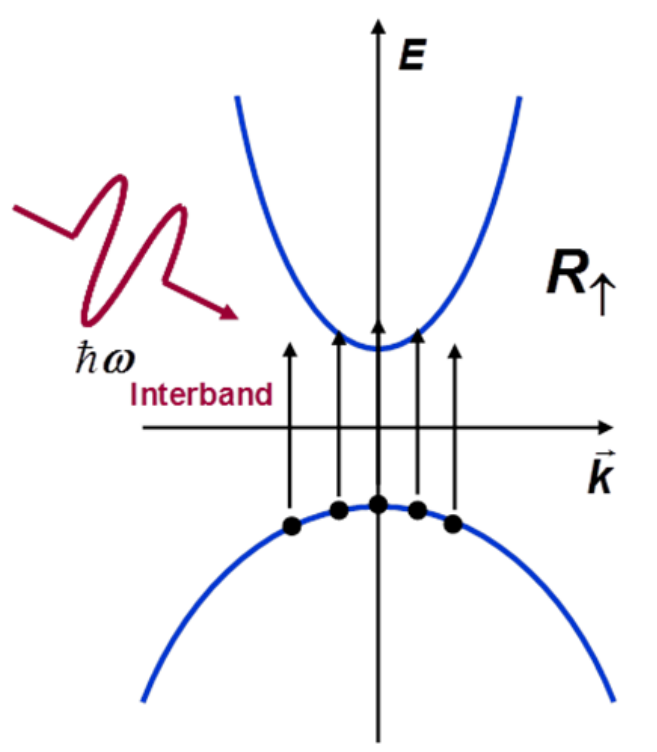
\includegraphics[height=2.0in,width=1.7in,viewport=0 0 630 760,clip]{Figures/Inter_band-transition_R.png}
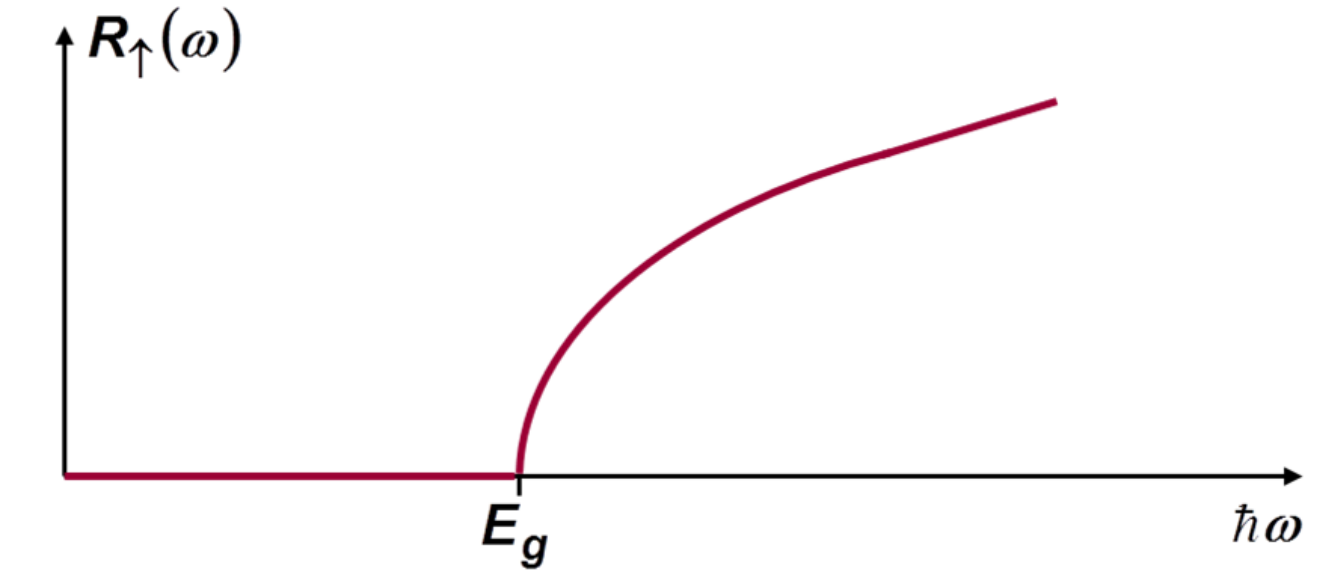
\includegraphics[height=1.0in,width=2.15in,viewport=0 0 1320 580,clip]{Figures/Inter_band-transition_JDOS.png}
\caption{\fontsize{5.2pt}{4.0pt}\selectfont\textrm{Schematic representation of the joint-DOS and the Van-Hove singularity.}}%
\label{Optic-JDOS}
\end{figure} 
}

\frame
{
	\frametitle{纵波电磁场下的电场与电子的相互作用}
仿照横波电磁场,以下讨论纵波电磁场下电子对电场的响应

用于描述电子的单电子\textrm{Hamiltonian}为
\begin{displaymath}
	H_0=\frac{\hbar^2{\nabla}^2}{2m}+V(\vec r)
\end{displaymath}

外加的波矢为$\vec q$频率为$\omega$微扰辐射为
\begin{displaymath}
	U(\vec r,t)=A_0\mathrm{e}^{\mathrm{i}(\vec q\cdot\vec r-\omega t)}+\mathrm{c.c.}
\end{displaymath}
这里$A_0=A_{\mathrm{tot}}(\vec q,\omega)$表示扰动的振幅

\textcolor{blue}{辐射场贡献的静电势}~(标量势)
\begin{displaymath}
	\phi(\vec r,t)=U(\vec r,t)/(-e)
\end{displaymath}
相应的\textcolor{red}{纵向电场$\mathbf{E}=-\nabla\phi$}
\begin{displaymath}
	\mathbf{E}(\vec r,t)=E_0\mathbf{e}\mathrm{e}^{\mathrm{i}(\vec q\cdot\vec r-\omega t)}+\mathrm{c.c}\quad\textcolor{red}{\mathbf{e}\parallel\vec q}
\end{displaymath}
并有$E_0=\mathrm{i}qA_0/e$,\textcolor{blue}{电场矢量与波矢方向平行}
}

\frame
{
	\frametitle{纵波电磁场下的电场与电子的相互作用}
微扰体系的\textrm{Hamiltonian}
\begin{displaymath}
	H=H_0+A_0\mathrm{e}^{\mathrm{i}(\vec q\cdot\vec r-\omega t)}+A_0^{\ast}\mathrm{e}^{-\mathrm{i}(\vec q\cdot\vec r-\omega t)}
\end{displaymath}
\textcolor{violet}{微扰项的存在将诱导$H_0$的本征态中的电子发生跃迁},两个微扰项分别伴随能量$\hbar\omega$的吸收和释放

根据标准\textrm{Fermi-golden}法则,单位时间内发生的全部吸收-释放过程,对应的能量(功率)
{\fontsize{9.0pt}{6.2pt}\selectfont{
\begin{displaymath}
\begin{aligned}
P(\vec q,\omega)=&\hbar\omega W(\vec q,\omega)\\
=&\hbar\omega\times\frac{2\pi}{\hbar}\textcolor{blue}{2}\sum_{\alpha,\beta}|\langle\psi_{\beta}|A_0\mathrm{e}^{\mathrm{i}\vec q\cdot\vec r}|\psi_{\alpha}\rangle|^2\delta(E_{\beta}-E_{\alpha}-\hbar\omega)[f(E_{\alpha})-f(E_{\beta}))]\\
=&4\pi\omega|A_0|^2\sum_{\alpha,\beta}|\langle\psi_{\beta}|\mathrm{e}^{\mathrm{i}\vec q\cdot\vec r}|\psi_{\alpha}\rangle|^2\delta(E_{\beta}-E_{\alpha}-\hbar\omega)[f(E_{\alpha})-f(E_{\beta}))]
\end{aligned}
\end{displaymath}}}
与横波电磁场中的推导类似
\begin{itemize}
	\item $\delta$因子表示跃迁过程的能量守恒关系
	\item 系数\textcolor{blue}{$2$}表示自旋简并态求和
\end{itemize}
}

\frame
{
	\frametitle{纵向介电函数\textrm{(longitudinal dielectric function)}}
	介质中由静电势$\phi$产生的电场$\mathbf{E}(\vec r,t)$,将产生传导电流
	\begin{displaymath}
		\mathbf{J}(\vec r,t)=\sigma(\vec q,\omega)E_0\mathbf{e}\mathrm{e}^{\mathrm{i}(\vec q\cdot\vec r-\omega t)}+\mathrm{c.c}\quad(\textcolor{red}{\mathbf{e}\parallel\vec q})
	\end{displaymath}
	传导电流$\mathbf{J}$单位时间消耗的能量为$\int_V\mathbf{J}\cdot\mathbf{E}\mathrm{d}\vec r$,因此有
由此计算得到吸收功率
{\fontsize{8.2pt}{6.2pt}\selectfont{
\begin{displaymath}
	\begin{aligned}
		\int_V\mathbf{J}\cdot\mathbf{E}\mathrm{d}\vec r=&\int_V[\sigma(\vec q,\omega)E_0\mathrm{e}^{\vec q\cdot\vec r-\omega t}+\mathrm{c.c}][E_0\mathrm{e}^{\vec q\cdot\vec r-\omega t}+\mathrm{c.c}]\mathrm{d}\vec r=\sigma(\vec q,\omega)|E_0|^2V+\mathrm{c.c}\\
		=&2\sigma_{\textcolor{blue}{1}}(\vec q,\omega)|E_0|^2V=2\sigma_1(\vec q,\omega)\frac{q^2}{e^2}|A_0|^2V=\textcolor{blue}{\hbar\omega W(\vec q,\omega)}
	\end{aligned}
\end{displaymath}}}
因此得到电导率的实部
\begin{displaymath}
	\sigma_1(\vec q,\omega)=\frac12\frac{e^2}{q^2}\frac{\hbar\omega W(\vec q,\omega)}{|A_0|^2V}
\end{displaymath}
于是纵向介电函数的虚部为
\begin{displaymath}
	\varepsilon_2(\vec q,\omega)=\frac{8\pi^2e^2}{q^2V}\sum_{\alpha\beta}|\langle\psi_{\beta}|\mathrm{e}^{\mathrm{i}\vec q\cdot\vec r}|\psi_{\alpha}\rangle|^2\delta(E_{\beta}-E_{\alpha}-\hbar\omega)[f(E_{\alpha})-f(E_{\beta})]
\end{displaymath}
}

\frame
{
	\frametitle{纵向介电函数\textrm{(longitudinal dielectric function)}}
	利用介电函数虚部-实部变换的\textrm{(Kramers-Kronig)}关系
	\begin{displaymath}
		\varepsilon_1(\vec q,\omega)=1+\frac1{\pi}\mathscr{P}\int_{-\infty}^{+\infty}\frac{\varepsilon_2(\vec q,\omega)}{\omega^{\prime}-\omega}\mathrm{d}\omega^{\prime}
	\end{displaymath}
介电函数的实部为
\begin{displaymath}
	\varepsilon_1(\vec q,\omega)=1+\frac{8\pi^2e^2}{q^2}\frac1V\sum_{\alpha\beta}|\langle\psi_{\beta}|\mathrm{e}^{\mathrm{i}\vec q\cdot\vec r}|\psi_{\alpha}\rangle|^2\frac{f(E_{\alpha})-f(E_{\beta})}{E_{\beta}-E_{\alpha}-\hbar\omega}
\end{displaymath}
因此纵向介电函数为
	\begin{displaymath}
		\varepsilon(\vec q,\omega)=1+\frac{8\pi^2e^2}{q^2}\frac1V\sum_{\alpha\beta}\frac{|\langle\psi_{\beta}|\mathrm{e}^{\mathrm{i}\vec q\cdot\vec r}|\psi_{\alpha}\rangle|^2}{E_{\beta}-E_{\alpha}-\hbar\omega-\mathrm{i}\eta}[f(E_{\alpha})-f(E_{\beta})]
	\end{displaymath}
}

\frame
{
	\frametitle{长波极限下的纵向与横向介电函数}
	在长波极限下$\vec q\rightarrow0$,此时介电函数的主要贡献来自
	\begin{displaymath}
		\langle\psi_{\beta}|\mathrm{e}^{\mathrm{i}\vec q\cdot\vec r}|\psi_{\alpha}\rangle=\mathrm{i}\vec q\cdot\langle\psi_{\beta}|\vec r|\psi_{\alpha}\rangle=\frac{\hbar}{m_e}\frac{\mathrm{i}\vec q\cdot\langle\psi_{\beta}|\vec p|\psi_{\alpha}\rangle}{E_{\beta}-E_{\alpha}}
	\end{displaymath}
	推导过程中利用了
	\begin{itemize}
		\item 将$\mathrm{e}^{\mathrm{i}\vec q\cdot\vec r}$展开到一阶
			\begin{displaymath}
				\mathrm{e}^{\mathrm{i}\vec q\cdot\vec r}=1+\mathrm{i}\vec q\cdot\vec r+\mathcal{O}(\vec q^2)
			\end{displaymath}
		\item 对易关系
			\begin{displaymath}
				[H_0,\vec r]=-\frac{\mathrm{i}\hbar}{m_e}\vec p
			\end{displaymath}
	\end{itemize}
	引入微扰电场极化矢量$\vec q$的方向$\mathbf{e}$,不难看出:\\
	\textcolor{purple}{长波极限下,纵向介电函数与横向介电函数趋于一致}
	\begin{displaymath}
		\varepsilon(\textcolor{blue}{0},\omega)=1+\frac{8\pi^2e^2}{m^2}\frac1V\sum_{\alpha\beta}\frac{|\langle\psi_{\beta}|\textcolor{red}{\mathbf{e}\cdot\vec p}|\psi_{\alpha}\rangle|^2}{[(E_{\beta}-E_{\alpha})/\hbar]^2}\frac{f(E_{\alpha})-f(E_{\beta})}{E_{\beta}-E_{\alpha}-\hbar\omega-\mathrm{i}\eta}
	\end{displaymath}
}

\frame
{
	\frametitle{长波极限下的光学函数的计算}
	原则上,横向介电函数的计算方案较为方便,但是横向介电函数推导时要求矢量场满足\textrm{Coulomb}规范:$\nabla\cdot\mathbf{A}=0$,这是一个大制约
	\begin{itemize}
		\item 横向介电函数的计算结果一般不如纵向介电函数
		\item 只有在局域势条件下,跃迁矩阵元计算才能利用对易关系简化
	\end{itemize}
	赝势方法中,由于存在非局域势,对易关系发生改变
	\begin{displaymath}
		[H,\vec r]=-\frac{\mathrm{i}\hbar}{m_e}\vec p+\textcolor{red}{\mathrm{i}[v_{\mathrm{nl}},\vec r]}
	\end{displaymath}
	\begin{itemize}
		\item \textcolor{blue}{全势方法的光学函数一般采用横向介电函数计算方案}
		\item \textcolor{violet}{赝势和\textrm{PAW}方法,光学函数主要采用纵向介电函数方案计算}
	\end{itemize}
}

\frame
{
	\frametitle{长波极限下的光学函数的计算}
	在$\vec k$空间计算纵向介电函数时,将遇到大量的跃迁矩阵元
	\begin{displaymath}
		\frac{\vec q}q\cdot\vec p_{\alpha\beta}=(E_{\alpha}-E_{\beta})\frac{m_e}{\hbar}\lim_{\vec q\rightarrow0}\bigg\langle\tilde\psi_{\alpha}\bigg|\frac1q\mathrm{e}^{\mathrm{i}\vec q\cdot\vec r}\bigg|\tilde\psi_{\beta}\bigg\rangle
	\end{displaymath}
	%$\langle\psi_{\vec k+\vec q}^{\beta}|\mathrm{e}^{\mathrm{i}\vec q\cdot\vec r}|\psi_{\vec k}^{\alpha}\rangle$和$\langle\psi_{\vec k+\vec q}^{\beta}|\psi_{\vec k}^{\alpha}\rangle$
	类型的积分,处理策略是
	\begin{itemize}
		\item 将$\mathrm{e}^{\mathrm{i}\vec q\cdot\vec r}$对$\vec q$展开到一阶
			\begin{displaymath}
				\mathrm{e}^{\mathrm{i}\vec q\cdot(\vec r-\vec R)}=1+\mathrm{i}\vec q\cdot(\vec r-\vec R)+\mathcal{O}(\vec q^2)
			\end{displaymath}
		\item 赝波函数$|\tilde\psi_{\vec k+\vec q}^n\rangle$利用\textrm{Bloch}定理处理周期函数$|\tilde{u}_{\vec k+\vec q}^n\rangle$,同样对$\vec q$展开到一阶
			\begin{displaymath}
				|\tilde u_{\vec k+\vec q}^n\rangle=|\tilde u_{\vec k}^n\rangle+\vec q\nabla_{\vec k}|\tilde u_{\vec k}^n\rangle+\mathcal{O}(\vec q^2)
			\end{displaymath}
		\item 在\textrm{PAW}方法中,投影函数$|\tilde p_{i,\vec k+\vec q}\rangle$也对$\vec q$展开到一阶
			\begin{displaymath}
				\tilde p_{i,\vec k+\vec q}\rangle=1-[\mathrm{i}\vec q(\vec r-\vec R_i)]|\tilde p_{i,\vec k}\rangle+\mathcal{O}(\vec q^2)
			\end{displaymath}
	\end{itemize}
	具体可参阅文献\cite{PRB73-045112_2006}
}

\subsection{复杂的光子与电子相互作用}
\frame
{
	\frametitle{电子对光子的吸收与受激辐射}
电子、空穴与相互作用	
\begin{figure}[h!]
\centering
%\hspace*{-10pt}
\vspace*{-0.2in}
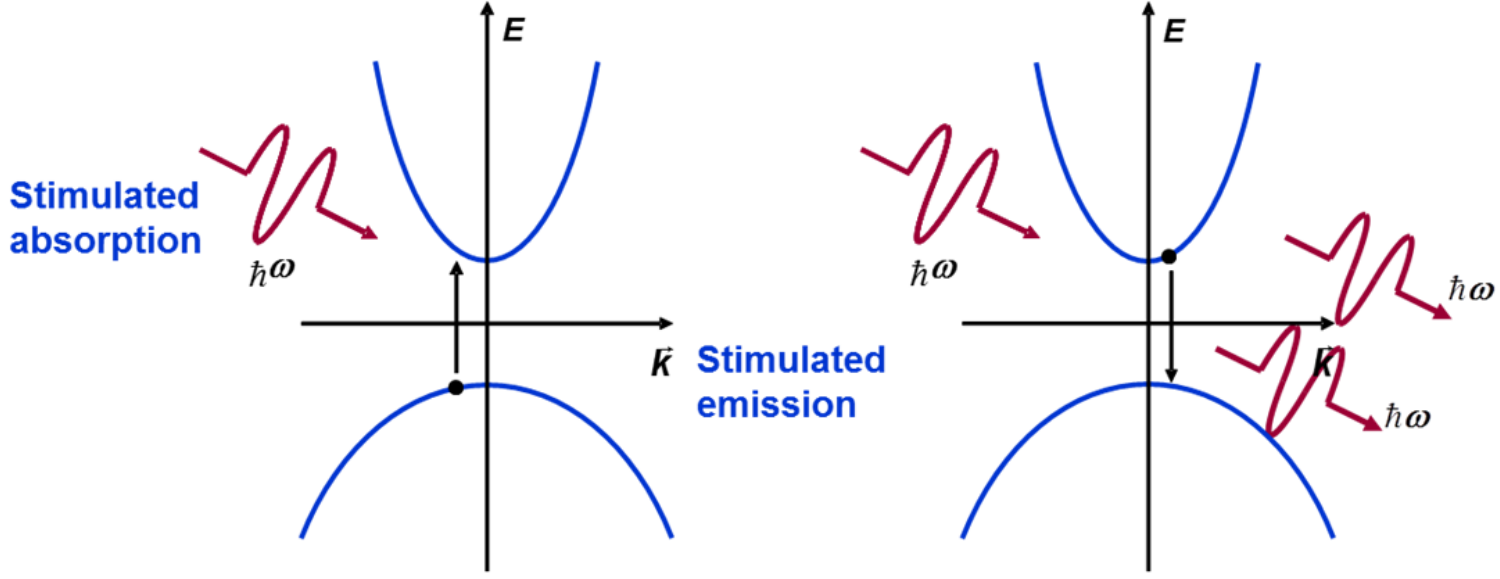
\includegraphics[height=1.9in,width=4.1in,viewport=0 0 1500 600,clip]{Figures/Inter_band-transition_abs-emi.png}
\caption{\fontsize{5.2pt}{4.0pt}\selectfont\textrm{Schematic representation of the stimulated absorption and emission of electrons.}}%
\label{Stimulated-absorption-emission}
\end{figure} 
电子-空穴对构成准粒子\textrm{(quasi-particle)}
}

\frame
{
	\frametitle{电子的自发辐射}
	电子-空穴的复合与准粒子的寿命
\begin{figure}[h!]
\centering
%\hspace*{-10pt}
\vspace*{-0.05in}
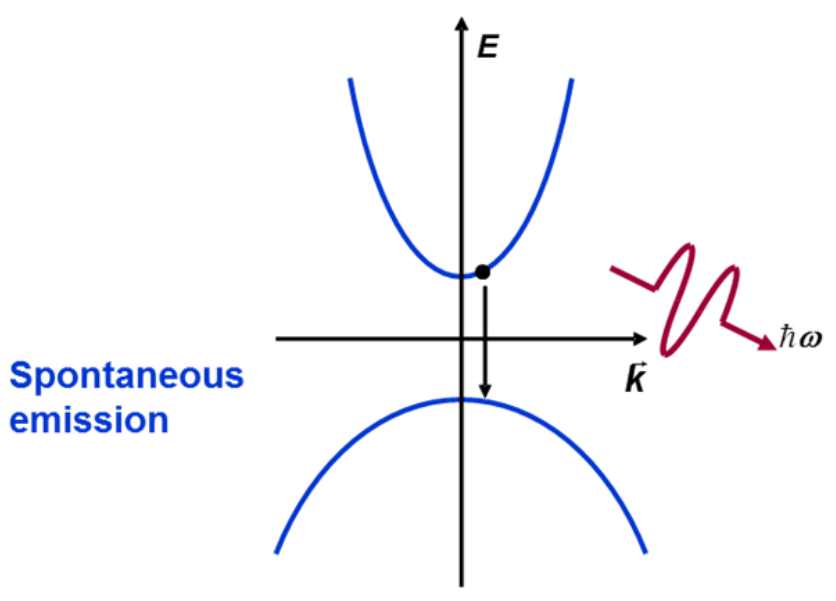
\includegraphics[height=2.0in,width=2.7in,viewport=0 0 830 620,clip]{Figures/Inter_band-transition_emission.png}
\caption{\fontsize{5.2pt}{4.0pt}\selectfont\textrm{Schematic representation of the spontaneous emission of electrons.}}%
\label{spontaneous-emission}
\end{figure} 
}

\frame
{
	\frametitle{复杂的系间窜越:~荧光、磷光与内转换}
\begin{figure}[h!]
\centering
%\hspace*{-10pt}
\vspace*{-0.05in}
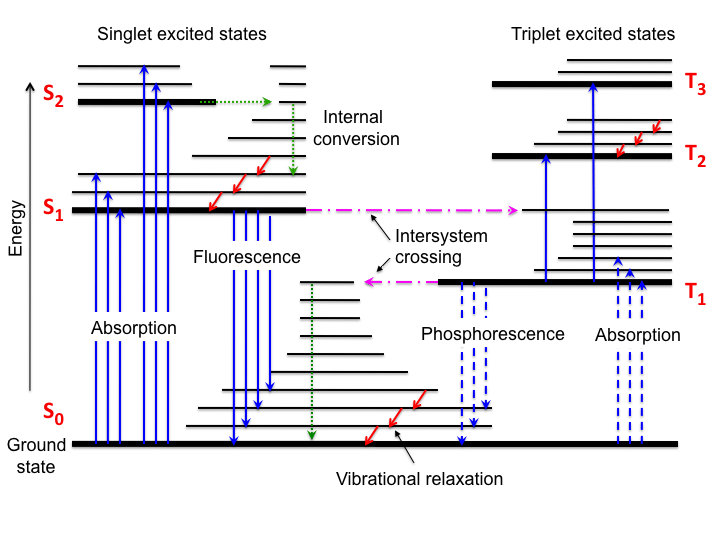
\includegraphics[height=2.3in,width=3.3in,viewport=0 0 720 520,clip]{Figures/Typical-diagram-of-the-electronic-energy-levels-of-a-molecule-with-singlet-and-triplet.png}
\caption{\fontsize{5.2pt}{4.0pt}\selectfont\textrm{Typical diagram of the electronic energy levels of a molecule with singlet and triplet  systems. The most important radiative (fluorescence and phosphorescence) and non-radiative (internal conversion, vibrational relaxation, intersystem crossing) transitions are shown.}}%
\label{singlet-triplet}
\end{figure} 
}

\frame
{
	\frametitle{吸收谱与发射谱}
\begin{figure}[h!]
\centering
%\hspace*{-10pt}
\vspace*{-0.19in}
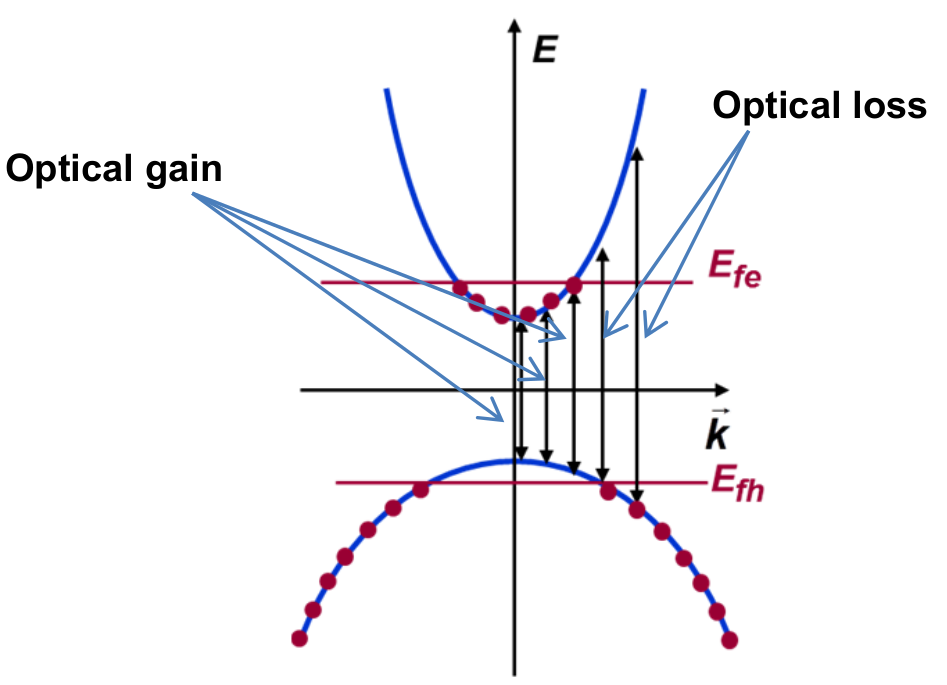
\includegraphics[height=2.5in,width=3.80in,viewport=0 0 950 700,clip]{Figures/Optical_gain-loss.png}
%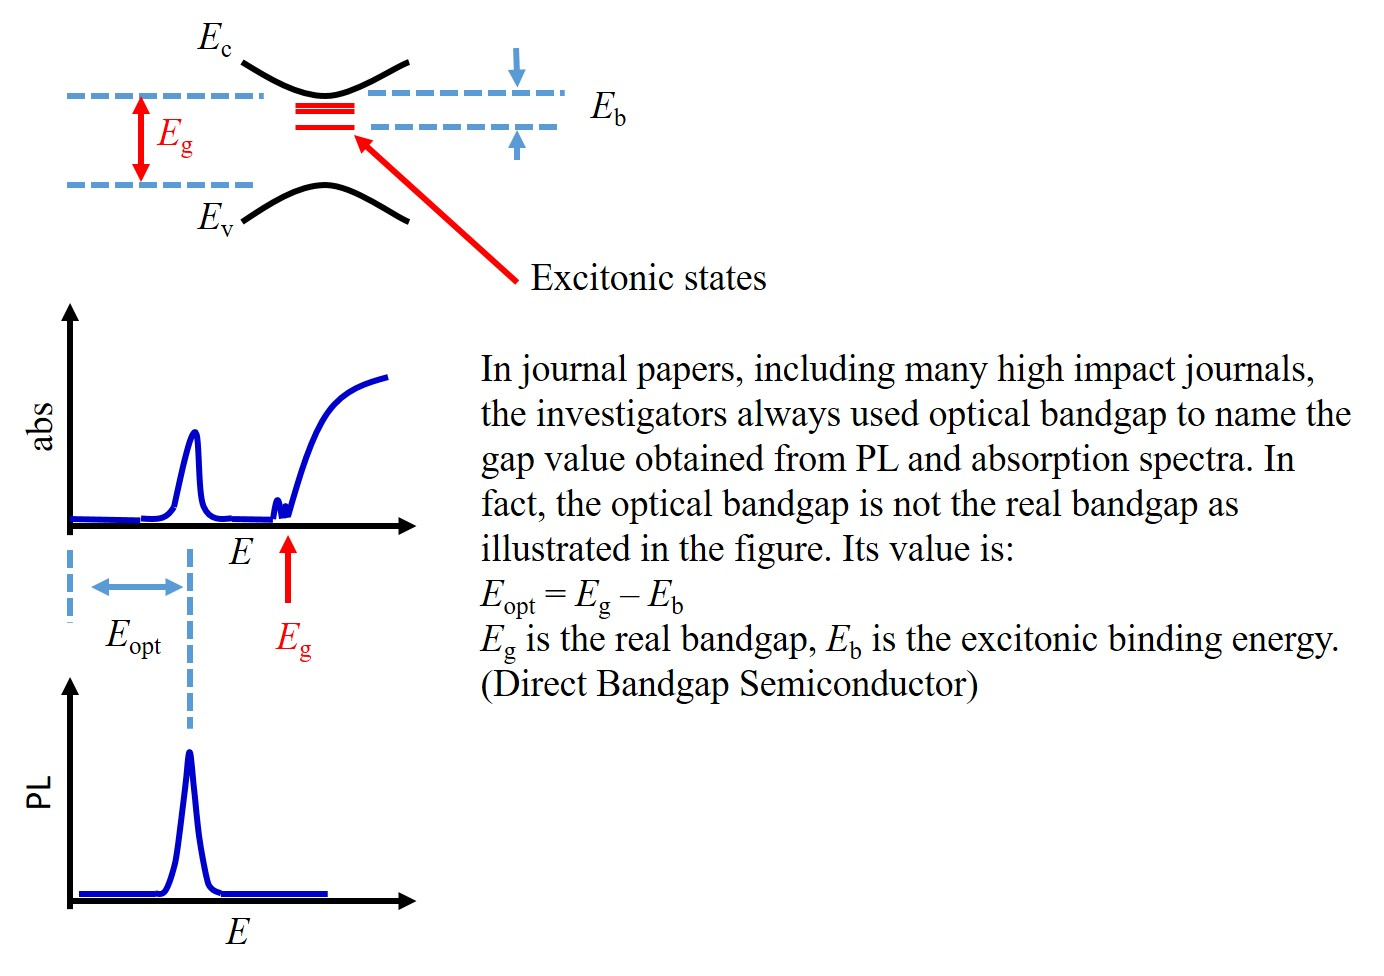
\includegraphics[height=1.1in,width=2.00in,viewport=0 0 670 460,clip]{Figures/Optical_Bandgap.jpg}
\caption{\fontsize{5.2pt}{4.0pt}\selectfont\textrm{Schematic representation of the gain-loss spectra.}}%
\label{gain-loss_Bandgap}
\end{figure} 
}

\frame
{
	\frametitle{光电子能谱与电子带隙}
\begin{figure}[h!]
\centering
%\hspace*{-10pt}
\vspace*{-3pt}
%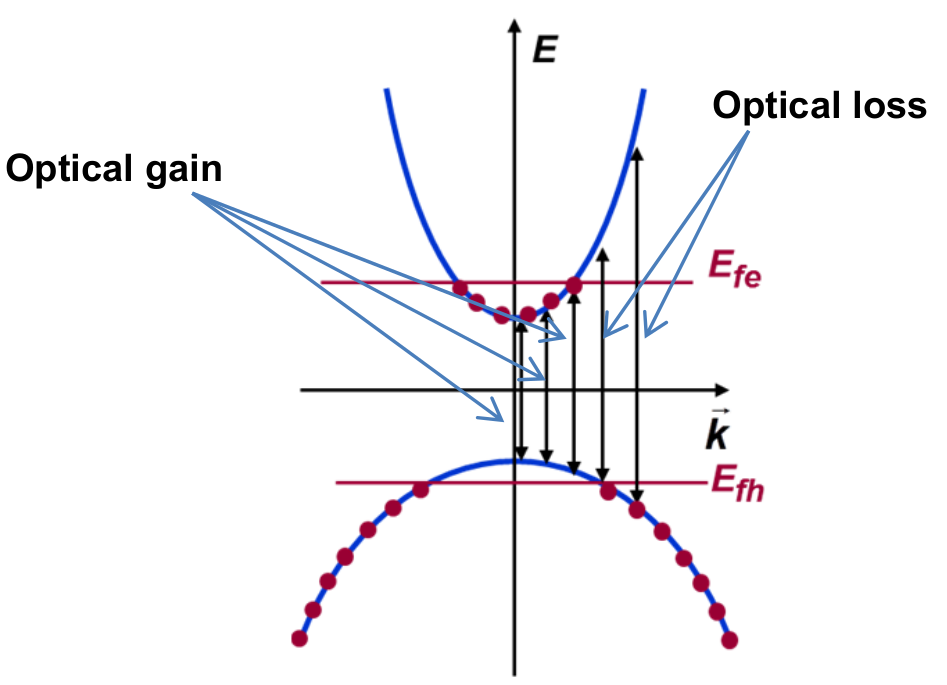
\includegraphics[height=1.7in,width=2.30in,viewport=0 0 950 700,clip]{Figures/Optical_gain-loss.png}
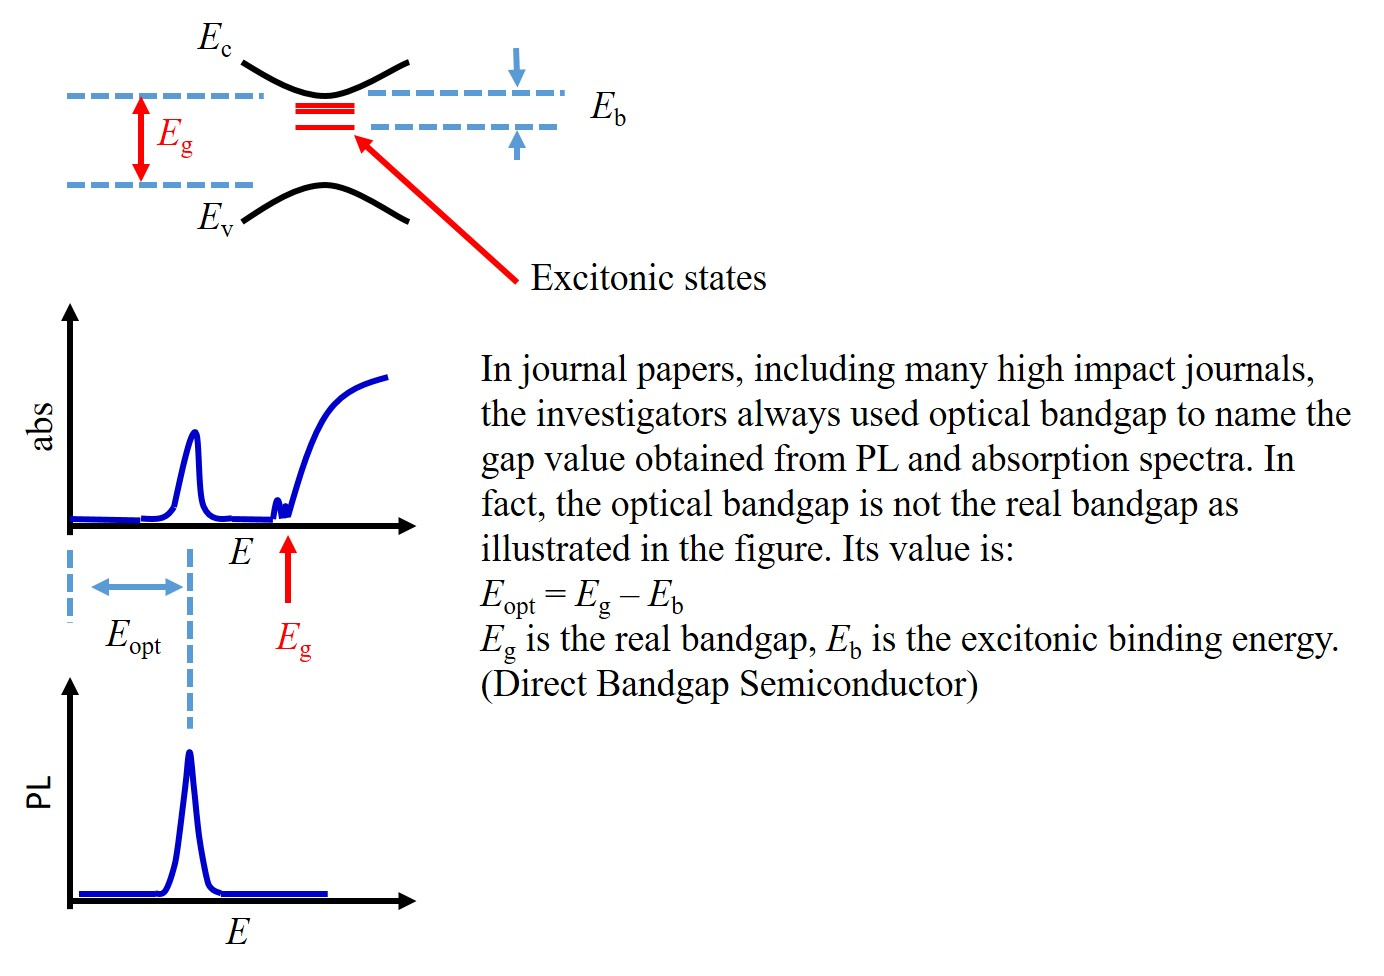
\includegraphics[height=2.4in,width=4.00in,viewport=0 0 670 460,clip]{Figures/Optical_Bandgap.jpg}
\caption{\fontsize{5.2pt}{4.0pt}\selectfont\textrm{Schematic representation of the spectra vs the band gap.}}%
\label{gain-loss_Bandgap}
\end{figure} 
}

%------------------------------------------------------------------------Reference----------------------------------------------------------------------------------------------
\begin{thebibliography}{99}
\frame[allowframebreaks]
{
\frametitle{主要参考文献}
{\tiny
\bibitem{PRB73-045112_2006}\textrm{M. Gajdo$\check{s}$, K. Hummer, G. Kresse, J. Furthm\"uller and F. Bechstedt. \textit{Phys. Rev.} B, \textbf{73} (2006), 045112}
}
\nocite*{}
}
\end{thebibliography}

